\subsubsection{Single Fungal Species}
It is simple to analyze and predict a single species of fungus, because in this ideal environment, the growth and reproduction process of a single fungus can be accurately represented by the \textbf{Logistic Model}. Substitute data of $F_A\sim F_E$ into the previous differential equation \textit{Eq.~(\ref{12eq})} and get \textit{Eq.~(\ref{14eq})} as follows.
\begin{equation}
  \label{14eq}
  \begin{cases}
    \frac{1}{N_A(t)}\frac{dN_A(t)}{dt} = r_A(1-\frac{N_A(t)}{{N_A}_{max}}) \\ \\
    \frac{1}{N_B(t)}\frac{dN_B(t)}{dt} = r_B(1-\frac{N_B(t)}{{N_B}_{max}}) \\ \\
    \frac{1}{N_C(t)}\frac{dN_C(t)}{dt} = r_C(1-\frac{N_C(t)}{{N_C}_{max}}) \\ \\
    \frac{1}{N_D(t)}\frac{dN_D(t)}{dt} = r_D(1-\frac{N_D(t)}{{N_D}_{max}}) \\ \\
    \frac{1}{N_E(t)}\frac{dN_E(t)}{dt} = r_E(1-\frac{N_E(t)}{{N_E}_{max}}) \\
  \end{cases}
\end{equation}
The function curves of $N_A(t)$, $N_B(t)$, $N_C(t)$, $N_D(t)$, and $N_E(t)$ are as follows.
\par
\begin{figure}[H]
  \centering
  \label{functioncurves}
  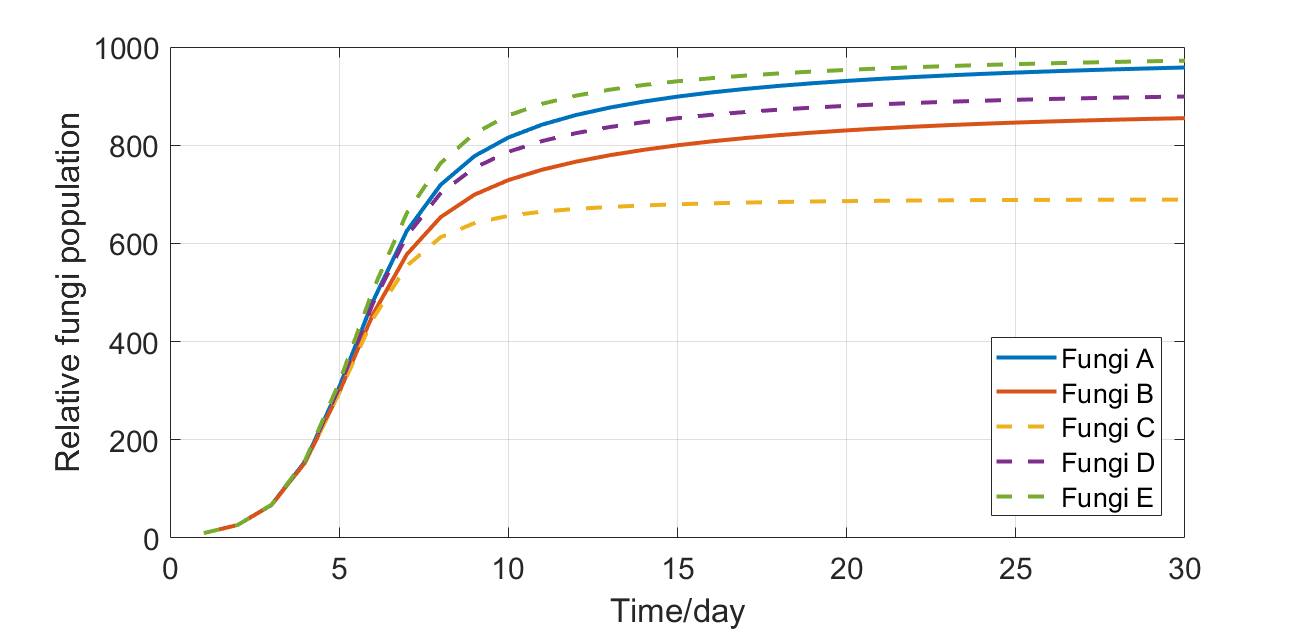
\includegraphics[width=\textwidth]{figures/Single.png}
  \caption{Function curves of each single fungus.}
\end{figure}
\par
The fungal data in the above figure are all based on the research and analysis of the environmental climate in \textit{Table~\ref{fivetypicalfungalspecies}}. The temperature, moisture and so on indicated in the table are the most suitable environmental conditions for the five fungi. Looking up the climatic data, it is found that the optimal growth environment of the five fungi corresponds exactly to the five typical climatic characteristics, including arid, semi-arid, temperate, arboreal and tropical rain forests. Therefore, it is obvious that when five species of fungi $F_A\sim F_E$, grow and reproduce under the optimal conditions, they can exert their greatest advantages in decomposing lignin or cellulose. On the contrary, these fungi will be at disadvantages due to excessive environmental blocking.
\begin{table}[H]
  \centering
  \caption{Corresponding optimal environment for the five fungi.}
  \label{correspondingoptimalenvironment}
  \begin{tabular*}{\hsize}{@{\extracolsep{\fill}}cccc}
    \toprule
    & Fungi & Corresponding Environment & \\
    \midrule
    & $F_A$ & Arid & \\
    & $F_B$ & Semi-arid & \\
    & $F_C$ & Temperate & \\
    & $F_D$ & Arboreal & \\
    & $F_E$ & Tropical rain forests & \\
    \bottomrule
  \end{tabular*}
\end{table}
The above table illustrates the corresponding optimal environment when the five fungi live alone, but it is quite different from the real situation in the nature. The following will further analyze the combinations between fungal species.